\documentclass[crop,tikz]{standalone}

% Field lines of an electric field inside and outside of a polarized
% sphere of radius R inside an infinitely large plate capacitor.
%
% The potential is independent of \varphi and is thus given by
%
% \phi(r,\theta) = -Ar\cos(\theta) + B\cos(\theta)/r^2,

% where A,B are given by the boundary conditions on the sphere:
% A=(\epsilon_r+2)/3E_i, B=(\epsilon_r-1)/3E_iR^3, where E_i is the
% field strength inside the sphere. So, the components of the electric
% field are
%
% E_r(r,\theta) = E_i\cos(\theta)[(\epsilon_r+2)/3+2(\epsilon_r)R^3/r^3/3],
% E_\theta(r,\theta) = -E_i\sin(\theta)[(\epsilon_r+2)/3-(\epsilon_r-1)R^3/r^3/3],
% E_z(r,\theta) = E_r(r,\theta)\cos(\theta)-E_\theta(r,\theta)\sin(\theta),
% E_y(r,\theta) = E_r(r,\theta)\sin(\theta)+E_\theta(r,\theta)\cos(\theta).

\usetikzlibrary{arrows.meta}

\usepackage{pgfplots}
\pgfplotsset{compat=1.18}

\pgfplotsset{
  inverted/.style = {
    every axis legend/.append style={
      draw=white,
      fill=hardblack,
      text=white
    }
  },
}

\begin{document}
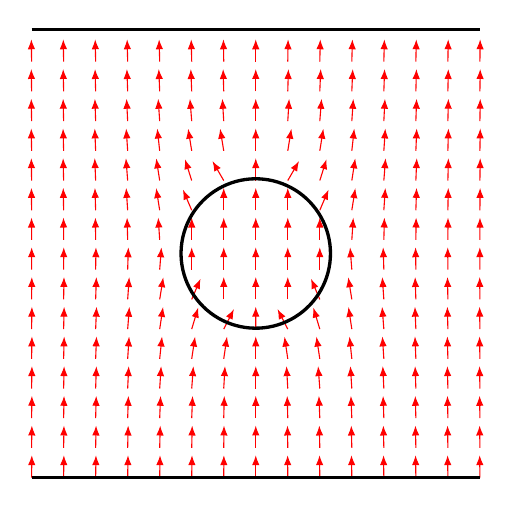
\begin{tikzpicture}
  \pgfmathsetmacro{\xmax}{3} % size of plot
  \pgfmathsetmacro{\R}{1.0} % radius of sphere
  \pgfmathsetmacro{\epsr}{4.0} % dielectric constant
  \pgfmathsetmacro{\Ei}{1.0} % field strength inside sphere
  \begin{axis}[
    view={0}{90},
    axis equal image,
    xmin={-\xmax}, xmax={\xmax},
    ymin={-\xmax}, ymax={\xmax},
    hide axis,
    clip=false,
    unbounded coords=discard,
    samples=15,
    samples y=15,
    declare function={
      rr(\x,\y) = sqrt(\x*\x + \y*\y);
      theta(\x,\y) = atan2(\y,\x);
      Er(\x,\y) = \Ei*cos(theta(\x,\y))*((\epsr+2)/3 + 2/3*(\epsr-1)*\R^3/(rr(\x,\y)^3));
      Etheta(\x,\y) = -\Ei*sin(theta(\x,\y))*((\epsr+2)/3 - (\epsr-1)/3*\R^3/(rr(\x,\y)^3));
      Ez(\x,\y) = Er(\x,\y)*cos(theta(\x,\y)) - Etheta(\x,\y)*sin(theta(\x,\y));
      Ex(\x,\y) = Er(\x,\y)*sin(theta(\x,\y)) + Etheta(\x,\y)*cos(theta(\x,\y));
      Ea(\x,\y) = sqrt(Ez(\x,\y)^2 + Ex(\x,\y)^2);
    },
    ]
    \addplot3[
      red,
      -{Latex[scale=0.75]},
      quiver={
        u={ifthenelse(rr(x,y)<\R, 0, Ex(x,y)/Ea(x,y))},
        v={ifthenelse(rr(x,y)<\R, 1, Ez(x,y)/Ea(x,y))},
        scale arrows=0.3,
      },
      domain=-3:3,
      domain y=-3:{3-2/15-0.3},
    ] ({x},{y},0);
    % sphere
    \addplot[black,very thick,domain=0:360,samples=100] ({\R*cos(x)}, {\R*sin(x)});
    % capacitor
    \draw[very thick] ({-\xmax},{\xmax}) -- ({\xmax},{\xmax});
    \draw[very thick] ({-\xmax},{-\xmax}) -- ({\xmax},{-\xmax});
  \end{axis}
\end{tikzpicture}
\end{document}
